\documentclass{kththesis}


%Taken from ID1354
\usepackage[utf8]{inputenc}
\usepackage[english]{babel}
\usepackage{graphicx}
\usepackage{lastpage}
\usepackage{pgf}
\usepackage{wrapfig}
\usepackage{fancyvrb}
\usepackage{fancyhdr}
\pagestyle{fancy}
\usepackage{dingbat}

\usepackage[autostyle]{csquotes}
\usepackage[
    backend=biber,
    style=ieee,
    sortlocale=de_DE,
    natbib=true,
    url=true,
    doi=true,
    eprint=false
]{biblatex}
\addbibresource{references.bib}

\usepackage[]{hyperref}
\hypersetup{
    colorlinks=true,
}

% List of abbreviations
\usepackage{glossaries}
\makeglossaries

\title{This is the English title}
\alttitle{Detta är den svenska översättningen av titeln}
\author{Jacob Kimblad}
\email{jacobki@kth.se}
\supervisor{Matthias Becker}
\examiner{Zhonghai Lu}
\programme{Master's Programme in Embedded Systems}
\school{School of Electrical Engineering and Computer Science}
\date{\today}


\begin{document}

%Term definitions
\newacronym{os}{OS}{Operating System}
\newacronym{cpu}{CPU}{Central Processing Unit}
\newacronym{lcu}{LCU}{Central Processing Unit}
\newacronym{aer}{AER}{Acquisition Execution Restitution}
\newacronym{cots}{COTS}{Commerical off the Shelf}
\newacronym{edf}{EDF}{Earliest Deadline First}
\newacronym{rms}{RMS}{Rate-Monotonic Scheduling}

% Frontmatter includes the title page, abstracts and table-of-contents
\frontmatter

\titlepage

\begin{abstract} 

    English abstract goes here.

\end{abstract}


\begin{otherlanguage}{swedish} 
    
    \begin{abstract}

    \end{abstract} 

\end{otherlanguage}

% List of Acronyms
\printglossary[title={Acronyms}]

% Table of contents
%\tableofcontents

% Mainmatter is where the actual contents of the thesis goes
\mainmatter


\chapter{Introduction} 
temp
Embedded systems in the automotive sector are required to go through a lot of analysis and testing
before being deemed safe for use in traffic. With the rise of autonomous vehicles these systems are
becoming more complex as an effect of more computing needed being done.  This has also put
requirements on the hardware to become faster and faster, thus the industry is turning to the use of
multi-core and many-core platforms. These type of platforms present more unpredictability than
single-core platforms which requires new methods of analysis and deterministic execution of these
systems. 


\section{Background} 

Timing analysis is an important part of real-time systems. However, multi-core platforms often
implement complicated memory hierarchies that make timing analysis a lot harder. One way to tackle
this is to schedule the access to shared memory in cooperation with computational tasks. This can
improve analysis and is employed by industrial domains already where the execution of tasks can be
divided up into three distinct parts, read-execute-write.


\section{Problem}

An analysis method for resource contention in multi-core real-time systems have been proposed in
paper [1]. This analysis method is however not 1 Template for project proposal 2018-12-12 customised
for the read-execute-write execution model that is adapted both within the avionics domain and
automotive domain.


\section{Purpose}

The purpose is to expand existing analysis methods by adding to the source code and/or produce a
model of the read-execute-write task model that is available as input for these formal analysis
methods.


\section{Goal}



\subsection{Benefits, Ethics and Sustainability}

\section{Methodology / Methods}

\section{Delimitations}

\section{Outline}


%We use the \emph{biblatex} package to handle our references.  We therefore use the command
%\texttt{parencite} to get a reference in parenthesis, like this \parencite{heisenberg2015}.  It is
%also possible to include the author as part of the sentence using \texttt{textcite}, like talking
%about the work of \textcite{einstein2016}.

\chapter{<Theoretic Background> Use a self-explaining title}



\section{The Task Model} \label{sec:the_task_model}

% TODO Center the text around tasks instead of jobs. Then explain how individual jobs can be
% modelled from the information given about its belonging task.

A periodic task, denoted as $T_j$ is a unit of work that is executed periodically on a processor
alongside other tasks over and over again where each iteration of execution is defined as a unique
job. In embedded systems a job is usually completed in some amount of time known as its execution
time, denoted as $C_i$, which is the same for all jobs in a task. Once a job is finished executing
the task will usually wait for some amount of time before its next job is ready to execute, this is
known as the tasks period. The largest-common-divider for all the tasks is known as the systems
hyper-period, defined as $H = lcm(period_j)$ for $i = 1, 2, ..., n$. For each multiple of a tasks
period a new job is released, this time is defined as the release time, denoted as $r_i$, and is
unique to each job within a single task. The job is also required to be finished before a set amount
of time from its release time, this is known as the jobs absolute deadline, denoted as $d_i$. For an
\acrshort{os} to decide in what order the jobs should be executed when more than one is available at
one time they are each assigned a priority, denoted as $p_i$, by a scheduler which is further
discussed in section \ref{sec:scheduling}.

A job can thus be defined by its characteristics as such $j_i = (r_i, C_i, d_i, p_i)$ where $j_i \in
T_j$ . And a task contains a set of jobs defines as $T_j = \{j_1, j_2, ..., j_n\}$ . It is then also
possible to define the set containing all of the jobs in the system the union all of the different
tasks $J = \{T_1 \cup T_2 \cup ... \cup T_m\}$ .

% TODO Add a one-sentence intro to pre-emption and tasks moved from running straight to ready

Following the above definitions we can ascribe properties to tasks telling us what state they are in
during a set time. After a job is released and is currently being executed the task which it belongs
to can be described as currently running. Once the job is finished and the next job from the same
task is yet to be released the task can be described as waiting before once again a job belonging to
the tasks starts executing and the task is running. Once a job is running it may require access to
some resource that is not ready to be accessed yet. Instead of the job taking up time on the
processor we can pause it and let some other job execute instead. We would then say that the task is
blocker. Once the resource is available again the task can be said to be ready before its job is
allowed to continue execution. The three different states that a task can be in depicted in figure
\ref{fig:ready-running-blocked-model}. 

% TODO reference to cyber-physical-systems? And follow their description

\begin{figure}

    \centering

    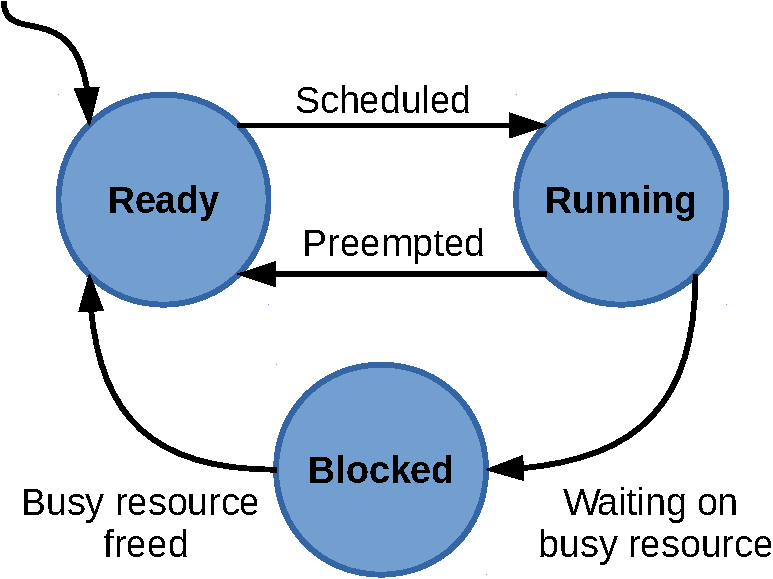
\includegraphics[width=0.5\linewidth]{images/ready-running-blocked-model.pdf}

    \caption{The three states a task may be in.}

    \label{fig:ready-running-blocked-model}

\end{figure}

% TODO: talk about aperiodic and sporadic tasks as well? 

\section{Scheduling} \label{sec:scheduling}

Although computers give away the illusion of being able to deal with very many things simultaneously
this is actually not the case. Computers are limited to how much parallel computing they are able to
do by the hardware, specifically the amount of cores within the \acrshort{cpu}. A computer with,
for example, four cores is only able to do at most four things in parallel at any one time. For a
computer to deal with more than four calculations requires switching ongoing calculations in and out
of a core. These calculations are often referred to as tasks and are discussed more in detail in
section \ref{sec:the_task_model}. For the \acrshort{os} to give an illusion of being able to execute
many tasks in parallel it needs to schedule the jobs of the tasks according to some order. This is
were the jobs priorities come in, by scheduling jobs and switching them in and out of the processor
very quickly depending on their priority the OS is able to perform many more calculations seemingly
at the same time than what is actually allowed for by hardware.

The order in which jobs are executed is determined by a scheduler which in of itself is a special
type of task executed by the \acrshort{os} of the system. The scheduler is invoked by the operating
system depending on different events in the system. It could for example be that a job is finished
executing or that it has begun waiting on some resource that is not yet available.  Different
scheduling algorithms are able to schedule same job sets unequally good, utilization is a
measurement introduced to compare how well schedulers actually work. The utilization of a scheduler
tells to what degree the scheduler is able to keep the processor busy for a given job set before
jobs start missing their deadlines. 

For embedded systems there exists a set of well known scheduling algorithms such as \acrshort{edf}
and \acrshort{rms}. Imagining a single-core \acrshort{cpu} the algorithm \acrshort{rms} works by
setting the priority of the jobs equal to the period of the task they are part of. This means that
the jobs belonging to the task with the lowest period are given the highest priority and always
scheduled first once they are ready. Since periods of tasks never changes during execution, the
priorities of the individual jobs belonging to a certain task will never change either, this is
known as fixed-priority scheduling. Instead of setting priorities according to the periods
\acrshort{edf} works by setting the priorities according to how close a job is to its deadline. T

\subsection{Multiprocessor scheduling}

\section{The AER Execution Model}

The \acrshort{aer} execution model was first proposed in \parencite{durrieu_predictable_2014} to
improve performance and predictability while using \acrshort{cots} multi-core processors with
distributed memory in the avionics industry. Since the bottleneck for these types of systems often
is the access to shared memory \acrshort{aer} focuses on making it more deterministic and easier to
analyse. This is done by dividing up the tasks that run within an \acrshort{os} into three distinct
parts.

%TODO Do we first explain what a task is, that it runs on a single core within a multi-processor and
%that for this industry it often is non-greedy when it is non-preemptive. Do we go into detail of
%the task model (running, ready and executing), this is probably good to cover in the global
%scheduling part.

The paper \parencite{maia_closer_2016} takes a closer look i


\chapter{<Engineering-related content, Methodologies and Methods> Use a self-explaining title}


\chapter{<The work> Use a self-explaining title}


\chapter{<Result> Use a self-explaining title}


\chapter{<Conclusions> Use a self-explaining title}


\printbibliography[heading=bibintoc] % Print the bibliography (and make it appear in the table of
    %contents)


\appendix

\chapter{Unnecessary Appended Material}


\end{document}
